\documentclass[border=4pt]{standalone}
\usepackage{tikz}
\usetikzlibrary{calc}
\usetikzlibrary{shapes.geometric}
\usetikzlibrary{arrows.meta}
\begin{document}

  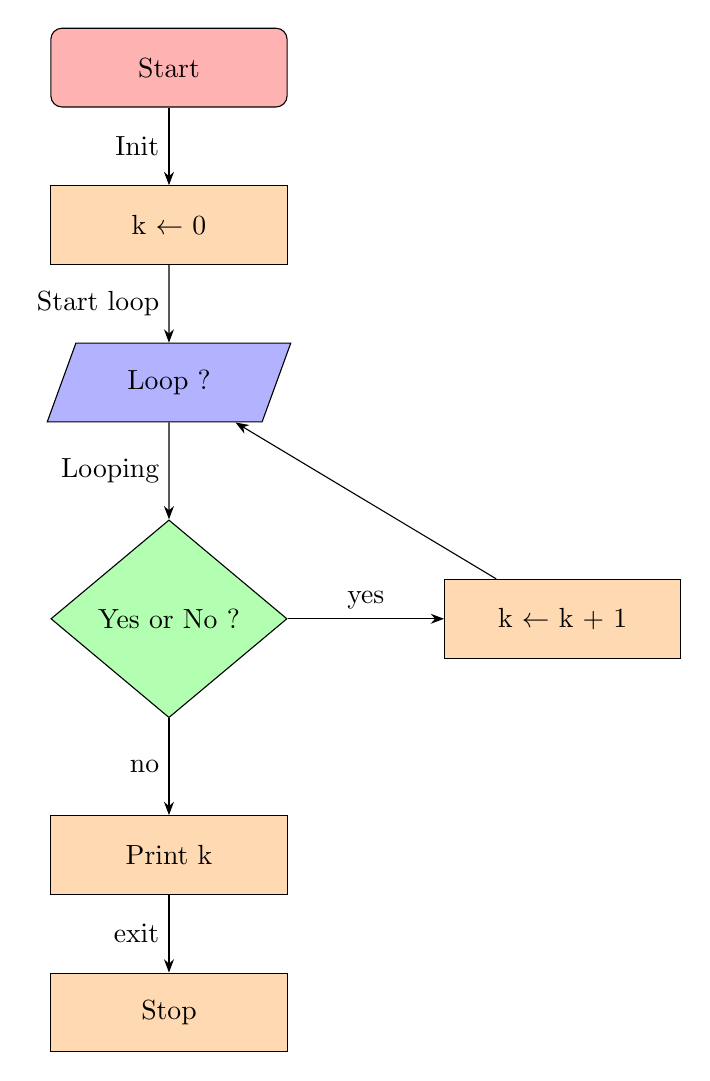
\begin{tikzpicture}[
    node distance=2cm,
    startstop/.style={rectangle, rounded corners, minimum width=3cm, minimum height=1cm,text centered, draw=black, fill=red!30},
    process/.style={rectangle, minimum width=3cm, minimum height=1cm, text centered, draw=black, fill=orange!30},
    io/.style={trapezium, trapezium left angle=70, trapezium right angle=110, minimum width=3cm, minimum height=1cm, text centered, draw=black, fill=blue!30},
    decision/.style={diamond, minimum width=3cm, minimum height=1cm, text centered, draw=black, fill=green!30},
    ]

    \node (node0) [startstop]                             {Start};
    \node (node1) [process, below of=node0]               {k $\leftarrow$ 0};
    \node (node2) [io, below of=node1]                    {Loop ?};     
    \node (node3) [decision, below of=node2, yshift=-1cm] {Yes or No ?};
    \node (node4) [process, right of=node3, xshift=3cm]   {k $\leftarrow$ k + 1};
    \node (node5) [process, below of=node3, yshift=-1cm]  {Print k};
    \node (node6) [process, below of=node5]               {Stop};

    \draw [arrows=-Stealth] (node3) --node[anchor=south]            {yes}        (node4);
    \draw [arrows=-Stealth] (node3) --node[anchor=east]             {no}         (node5);
    \draw [arrows=-Stealth] (node5) --node[anchor=east]             {exit}       (node6);
    \draw [arrows=-Stealth] (node2) --node[anchor=east]             {Looping}    (node3);
    \draw [arrows=-Stealth] (node1) --node[anchor=east]             {Start loop} (node2);
    \draw [arrows=-Stealth] (node0) --node[anchor=east]             {Init}       (node1);
    \draw [arrows=-Stealth] (node4) -- (node2);

  \end{tikzpicture}

\end{document}
